%! TEX root = ./master.tex

\lecture{20}{Week: 11}{Virtual Memory}


\subsubsection{Recap: Address Translation}
On most modern systems programs do not directly interact with the physical memory, but with its own virtual memory space. All these private virtual memory spaces are mapped on he physical memory.

\paragraph{Address Space}
The virtual/physical address space is a ordere set of contagious non-negative integer address from $0$ up to some $N - 1$. Where $N$ is determined by the system (bits) for virtual memory, and for physical memory by the size of the available memory.

Each virtual address must map to a physical address. A single physical address may be mapped to by multiple virtual addresses. This is useful for e.g. shared libraries.

Virtual memory is used in all modern computers. Only in simple systems like embedded mikrocontrollers physical addressing is still used.

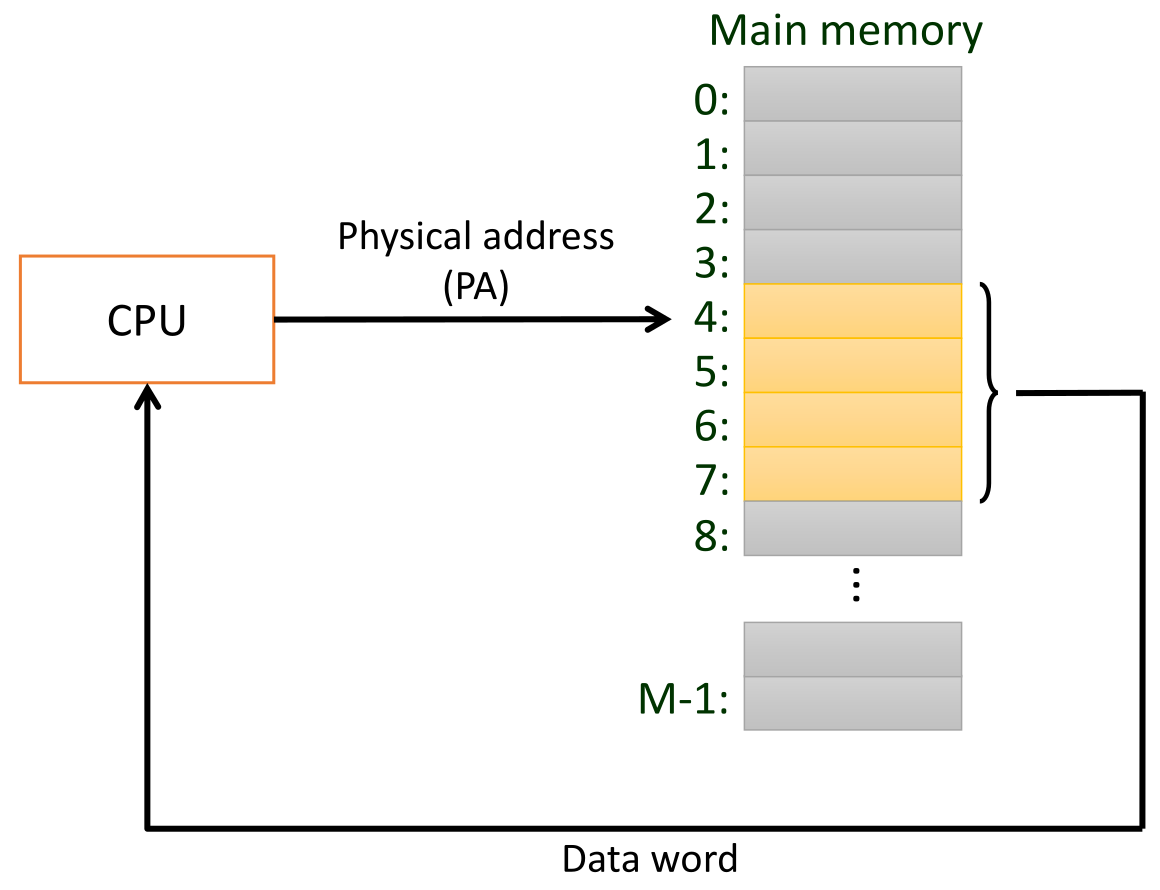
\includegraphics[width=0.8\textwidth]{20_physicalAddressing.png}

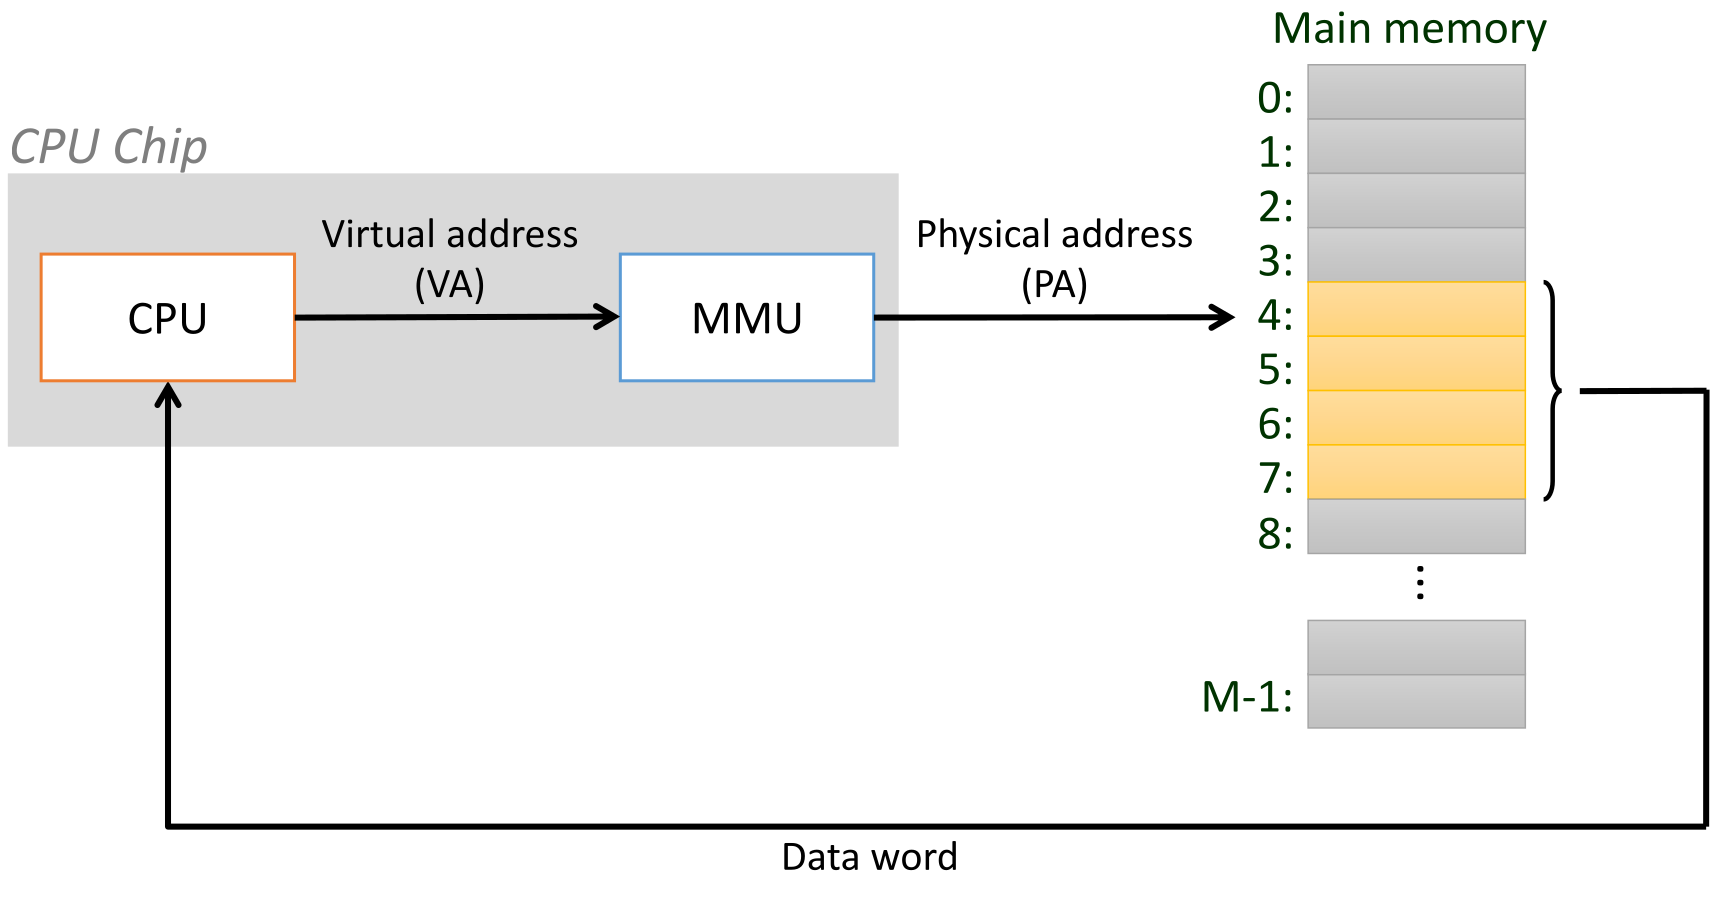
\includegraphics[width=0.8\textwidth]{20_virtualAddressing.png}

Virtual memory is handles by OS and hardware. We need hardware for a efficient translation. This is done by the memory management units (MMU). The translation table is managed by the OS.

\paragraph{Address Translation}
The OS operates on memory in blocks called pages. This is similar to caches and cache blocks. The default page size is 4KB. This size determines the granularity of the translation.

The translation is done using the page table. The table itself is stored in XXX and the start address is stored in the page table base register (PTBR). The start address is different for each process. The translation is done as as follows. The virtual address contains two parts, the \textit{Virtual Page Numer (VPN)} and the \textit{Virtual Page Offset (VPO)}. The VPN is taken and used to index into the page table. The entry gives uf the \textit{Physical Page Number (PPN)}. The PPN is concatenated with the unchanged VPO to get the physical address. An additional valid bit tells if the given VPN is valid or if it is not in memory (page fault).

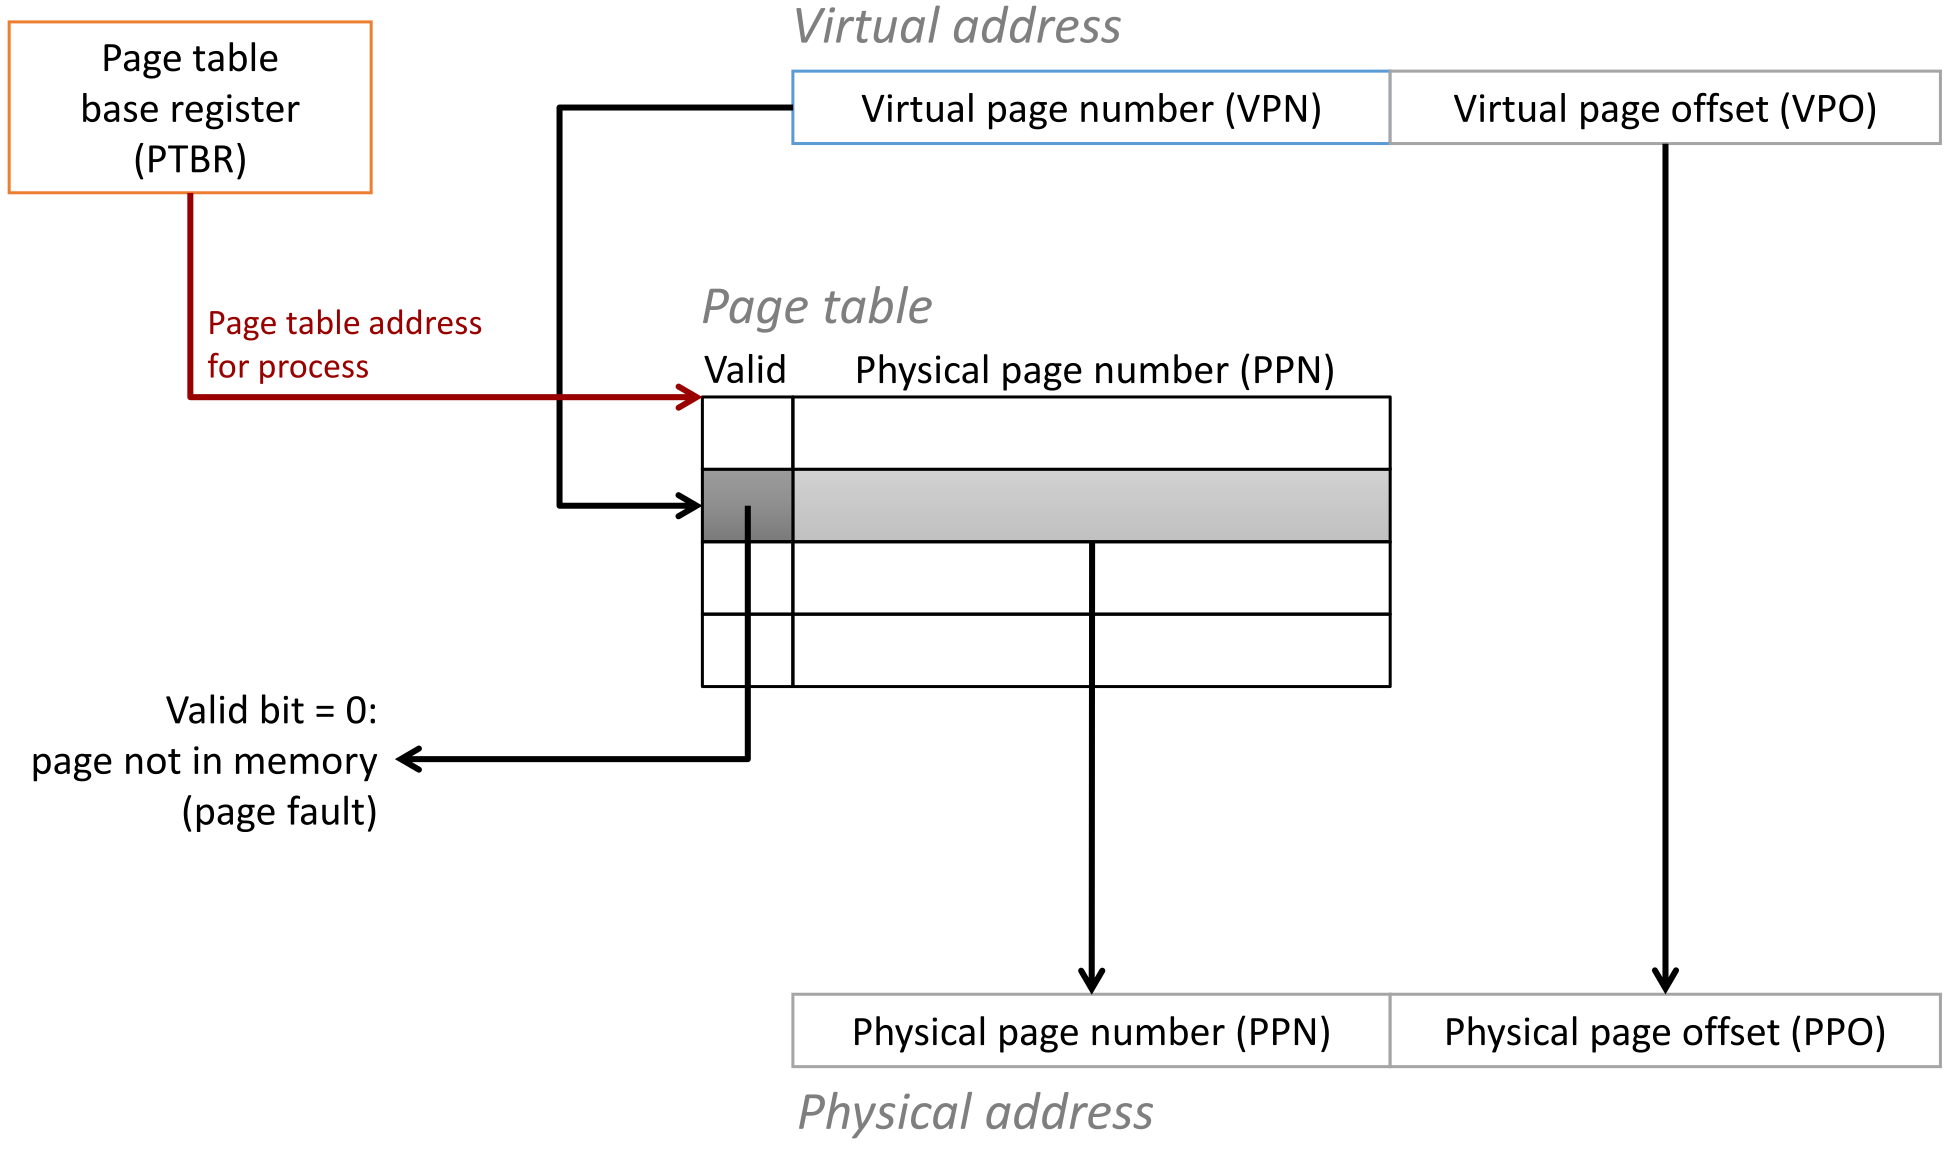
\includegraphics[width=0.8\textwidth]{20_translationProcedure.png}

\subsubsection{Uses of Virtual Memory}
\paragraph{Why Virtual Memory}
The use of VM has three main advantages:

\subparagraph{Efficient use of limited RAM}
Using $64$ bit addressing, we can address $16$ Exabytes of data. However, a commons system has only a few GB of RAM. So, VM provides a way to cache data by only storing parts of the virtual address space in disk and only keep active arias of virtual address space on memory. 

Memory pages can be in three different stages:
\begin{description}
    \item[Unallocated:] Page which was not yet used.
    \item[Cached:] Pages found on disk and on main memory.
    \item[Uncached:] Pages found on disk but not main memory.
\end{description}

Cached and uncached pages are found on disk. Additionally, cached  pages are also found on physical memory.

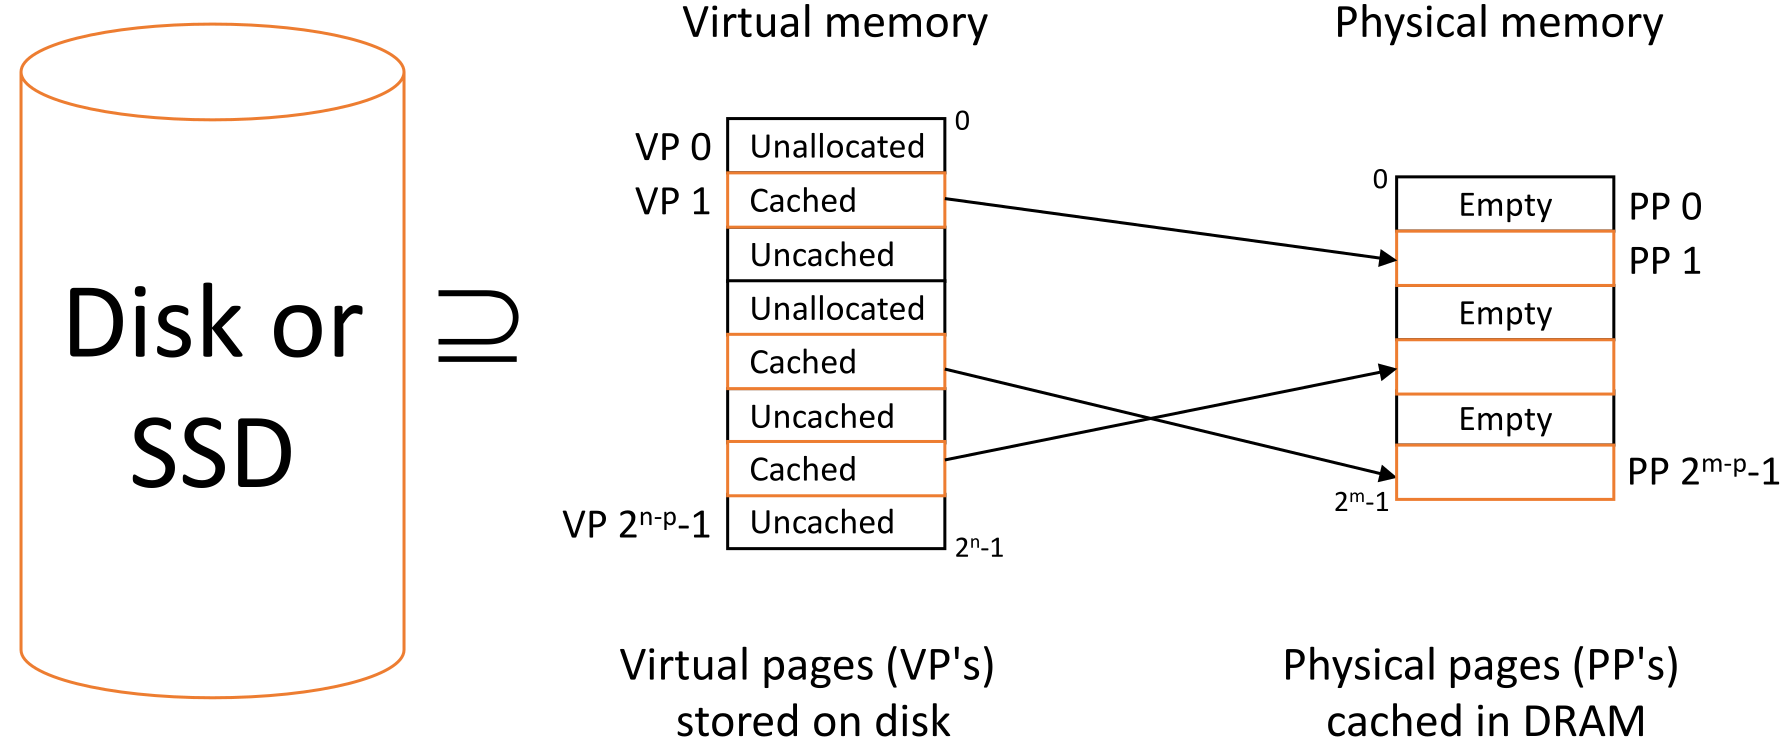
\includegraphics[width=0.8\textwidth]{20_cachingTool.png}

Since disk access is incredibly expensive, pages are larger then cache blocks to prevent going to cache too often. The process of bringing data (pages) from disk into memory is called paging or swapping. Replacement algorithms are highly sophisticated and therefore implemented in software. To further reduce the number of required paging, write-back policy is used instead of write-through.

This works thanks to locality. Meaning, the programs tend to access a set of active virtual pages, called the \textit{working set}. As long as the size of the working set is smaller than the main memory size, we can expect good performance. But as soon as it exceeds the memory size we get a performance meltdown, caused by copying and moving of pages.

Further, the smaller the page size, the more mappings we have. Since the \textit{Translation Lookaside Buffer (TLB)} is very small, only few mappings can be cached there. 

\subparagraph{Simplified memory management for programmers}
Each process gets a virtual address space of equal layout (i.e. heap, stack etc are located at the same addresses). The virtual address space is kind of a abstraction of the full memory mode. The linear virtual memory as actually scattered across the physical memory. But it is all managed by the OS.

\subparagraph{Protection and Sharing}
Virtual address spaces are isolated from each other different programs cannot interfere which each others memory. Besides that, PTE has some extra bits to tell if a physical memory location is readable, writable, executale or only accessible by superusers. The page fault hander checks these bits before remapping and causes a SIGSEGV exception in case they are violated.

\subparagraph{Simplifies linking and loading}
Since address spaces share the same layout. Linker precisely know at what address which section starts. This simplifies the implementation of linkers. 

Pages also allow for on dempand loading, where .data and .text are copied on demand. This improved loading efficiently greatly.


\subsubsection{Address Translation Process}

\paragraph{Page Hit}
The steps in case of a page hit are the following:
\begin{enumerate}
    \item The CPU sends the VM address to the MMU
    \item The MMU does a PTE access in the lookup table in the main memory
    \item The MMU receives the PTE from memory
    \item The MMU accesses the physical memory using the translated address
    \item The data is received and send to the CPU
\end{enumerate}

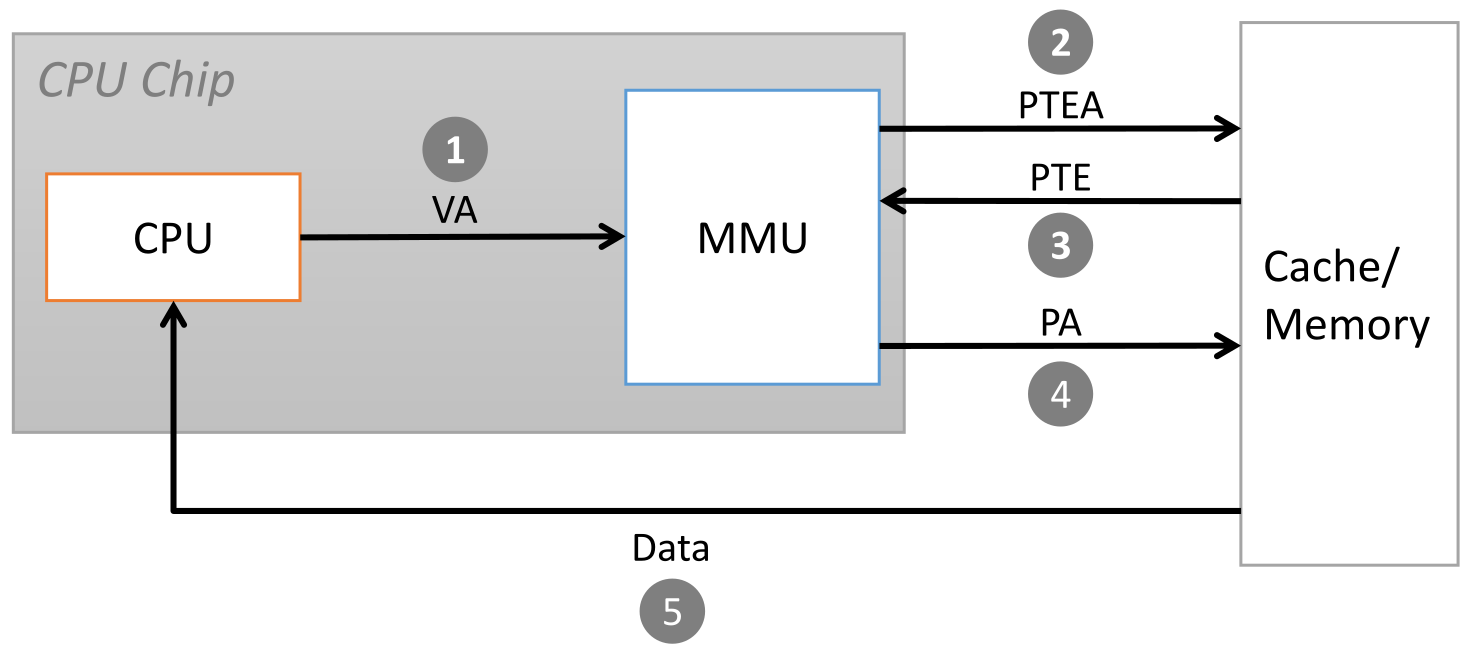
\includegraphics[width=0.8\textwidth]{20_pageHit.png}

These steps are all handled by HW.

\paragraph{Page Fault}
If the page is not cached, but uncached we have a miss (get a page fault) and have to fetch the data from disk.

\begin{enumerate}
    \item The CPU sends the VM address to the MMU
    \item The MMU does a PTE access in the lookup table in the main memory
    \item The MMU receives the PTE from memory
    \item The valid bit of the PTE is zero and so, the MMU trigger a page fault exception.
    \item The exception handler gets active and decides on a page to evict (to make space for the new page). Before evicting the page, it must check the dirty bit and depending on if it is set, write the page first back to disk.
    \item The handler pages (load page from memory) the new page and updates the PTE in memory.
    \item The handler returns to the original process and restarts the faulty instruction.
\end{enumerate}

The page fault hander is implemented in OS since it is more sophisticated.

\subsubsection{Translation Lookaside Buffers (TLB)}
Since the page table is stored in memory as all other data, PTEs gets also cached in the cache hierarchy. However, PTEs may get evicted by other data reference. Also, while L1 cache is quite fast, it still takes a few cycles. 

The \textit{Translation Lookaside Buffer (TLB)} solves this problem. It is a small hardware cache in the MMU and caches mappings of virtual page number ot physical page numbers. For small page tables, it may even contain the complete table.

TLB are very common.

\paragraph{TLB Hit}
In case the translation mapping in in the TLB, the following steps are executed.

\begin{enumerate}
    \item The CPU sends the VM address to the MMU
    \item The MMU indexes the TLB using the VPN bits
    \item From the TLV it receives the PTE bits
    \item The MMU concatenates the PTE and address offset and accesses and accesses the memory.
    \item The data is received and send to the CPU.
\end{enumerate}

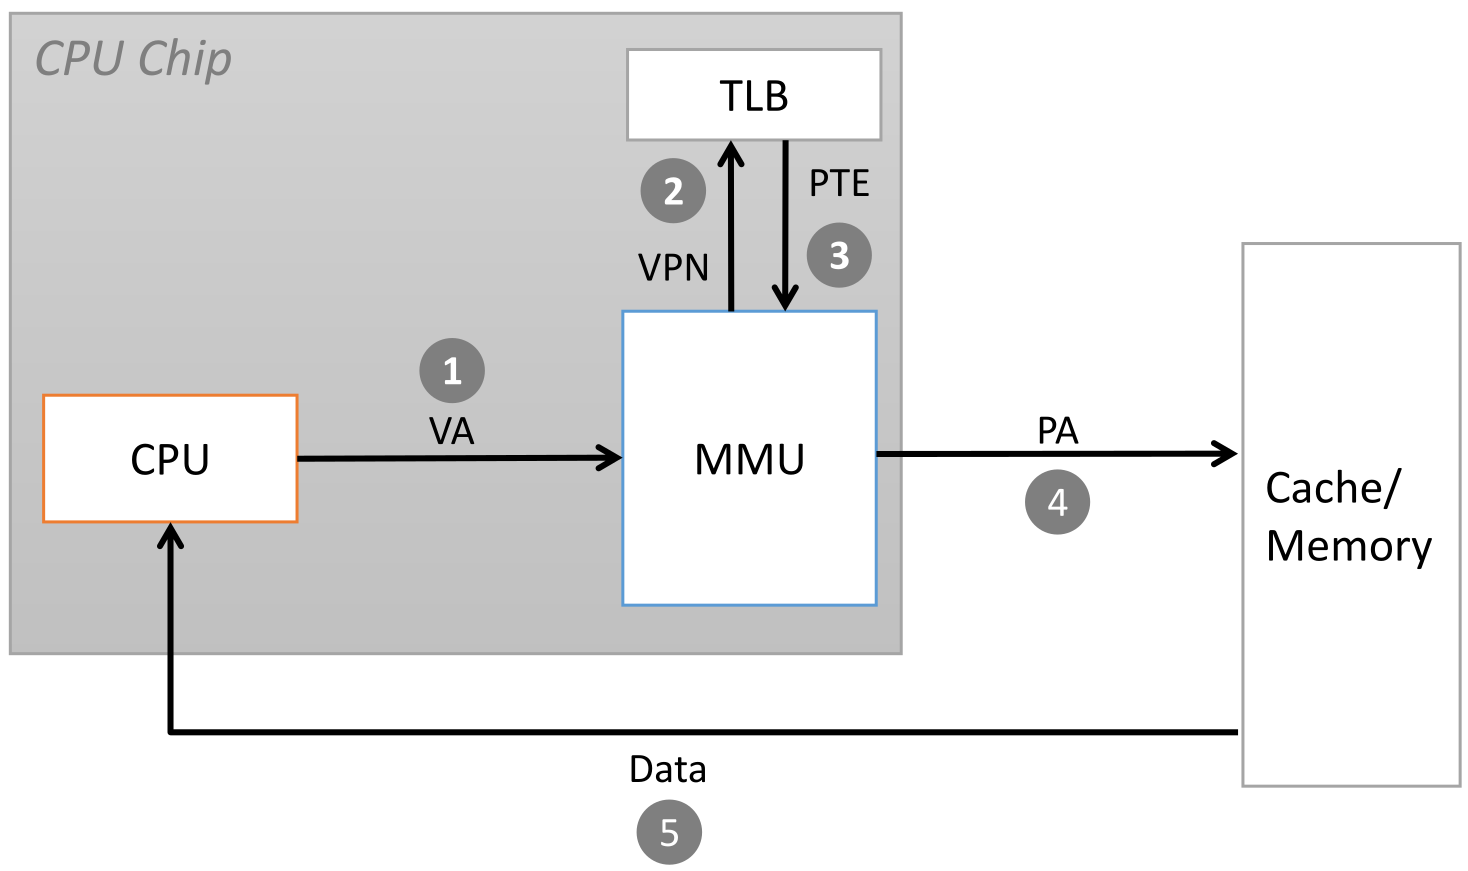
\includegraphics[width=0.8\textwidth]{20_TlbHit.png}

A hit eliminates an additional memory access to get the PTE.

\paragraph{TLB Miss}
If the VPN is not in TLB, me steps are:

\begin{enumerate}
    \item The CPU sends the VM address to the MMU
    \item The MMU indexedthe LTB using the VPN bits. But VPN is not in the TLB and therefore we do not get anything back.
    \item The MMU does a PTE access in the lookup table in the main memory
    \item The MMU receives the PTE from memory and puts it into the TLB (for further accesses to this page). receives the PTE from memory and puts it into the TLB (for further accesses to this page).
    \item The MMzu accesses the physical memory using the translated address
    \item The data is receive and send to the CPU
\end{enumerate}

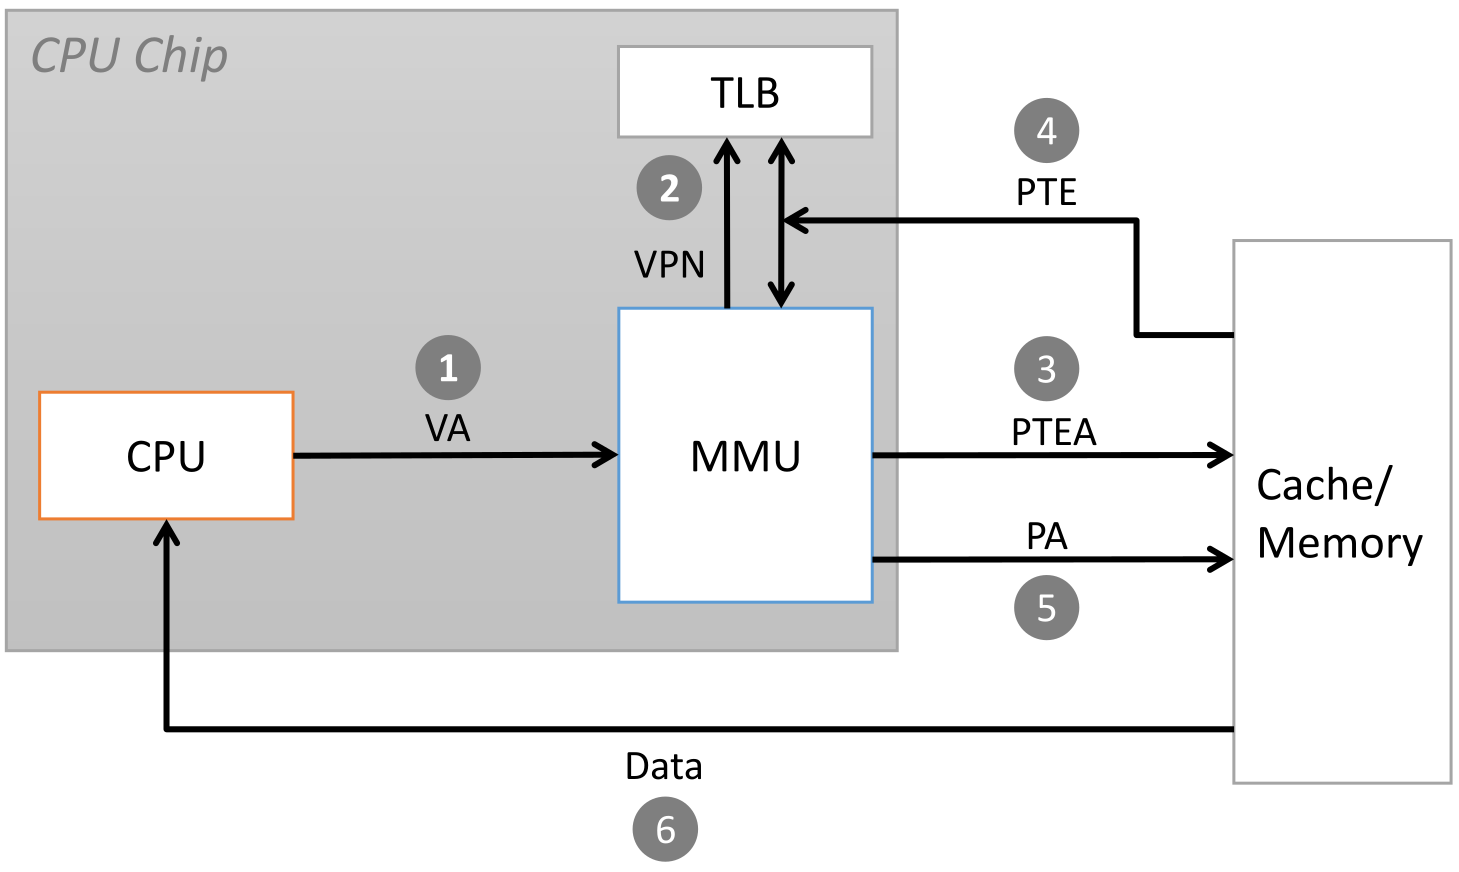
\includegraphics[width=0.8\textwidth]{20_TlbMiss.png}

TLB misses are actually rather rare.

\subsubsection{Simple Memory System Example}

\paragraph{Addressing}
Let's consider a memory system with $14$-bit virtual addresses and $12$-bit physical addresses and a page size of $64$ bytes. The size of the VPN, VPO, PPN and PPO is visible in the following graphic:

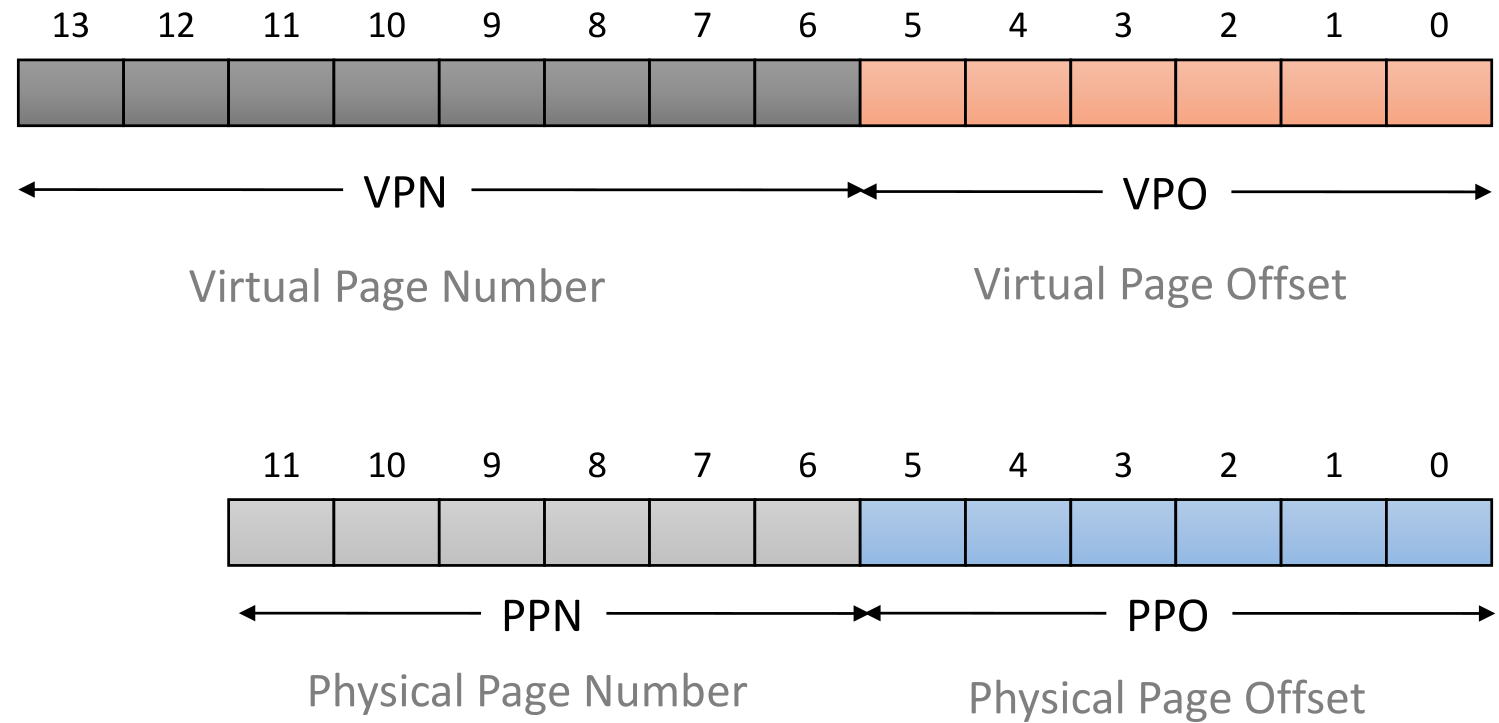
\includegraphics[width=0.8\textwidth]{20_exMemorySystem.png}

\paragraph{Page Table}
The first $16$ of total $256$ entries of the page table are:

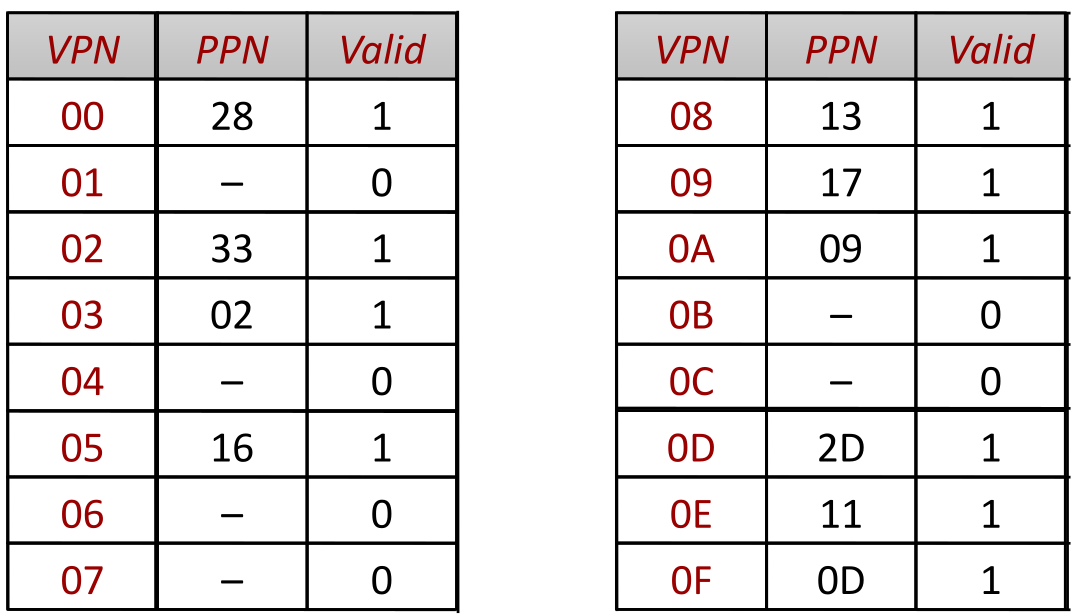
\includegraphics[width=0.8\textwidth]{20_exPageTable.png}

\paragraph{TLB}
The TLB contains $16$ entries and is $4$-way associative. The VPN is used to index into the TLB. The $2$ LSB of the VPN, the TLB index (TLBI), are used to determine the set of the TLB to use, and the remaining bits of the VPN, the TLB tyg (TLBT), are used to verify the tag of the TLB entry.

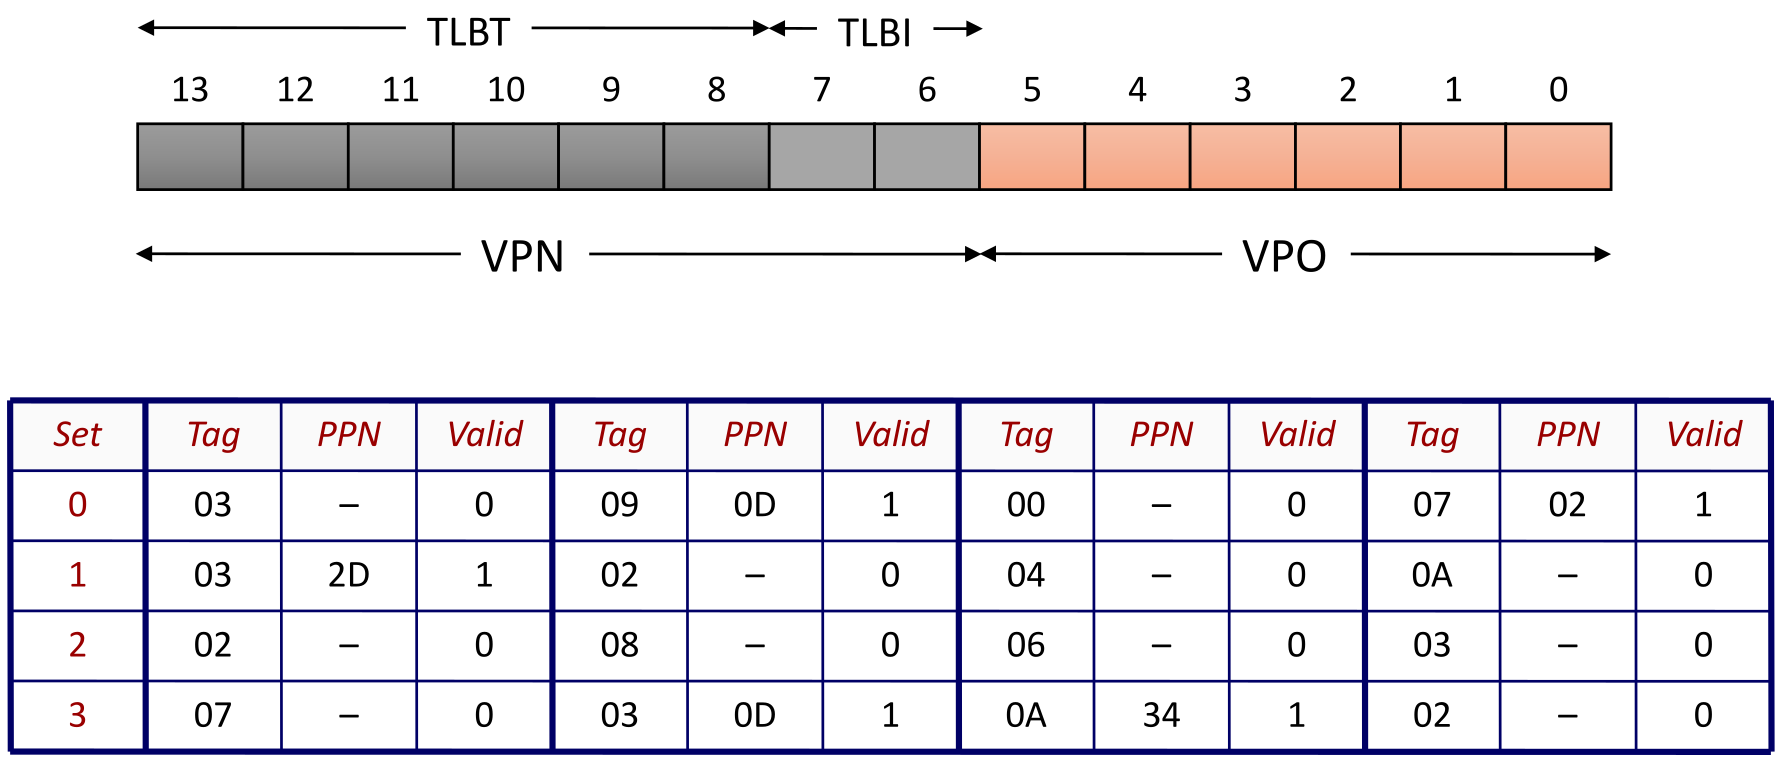
\includegraphics[width=0.8\textwidth]{20_ex_Tlb.png}

\paragraph{Cache}
The cache contains $16$ lines of each $4$-byte blocks size. The cache is addressed using physical addresses and it is directly mapped.

The physical address is split into three parts. The most significant $4$ bits of the PPO are used for the cache index (CI) and the remaining two for the cache offset (CO). The CI tells which index of the cache we want, and the CO determines in wich blocks we are actually interested. The full PPN is used as the cache tag (CT) to determine if we have a match or not.

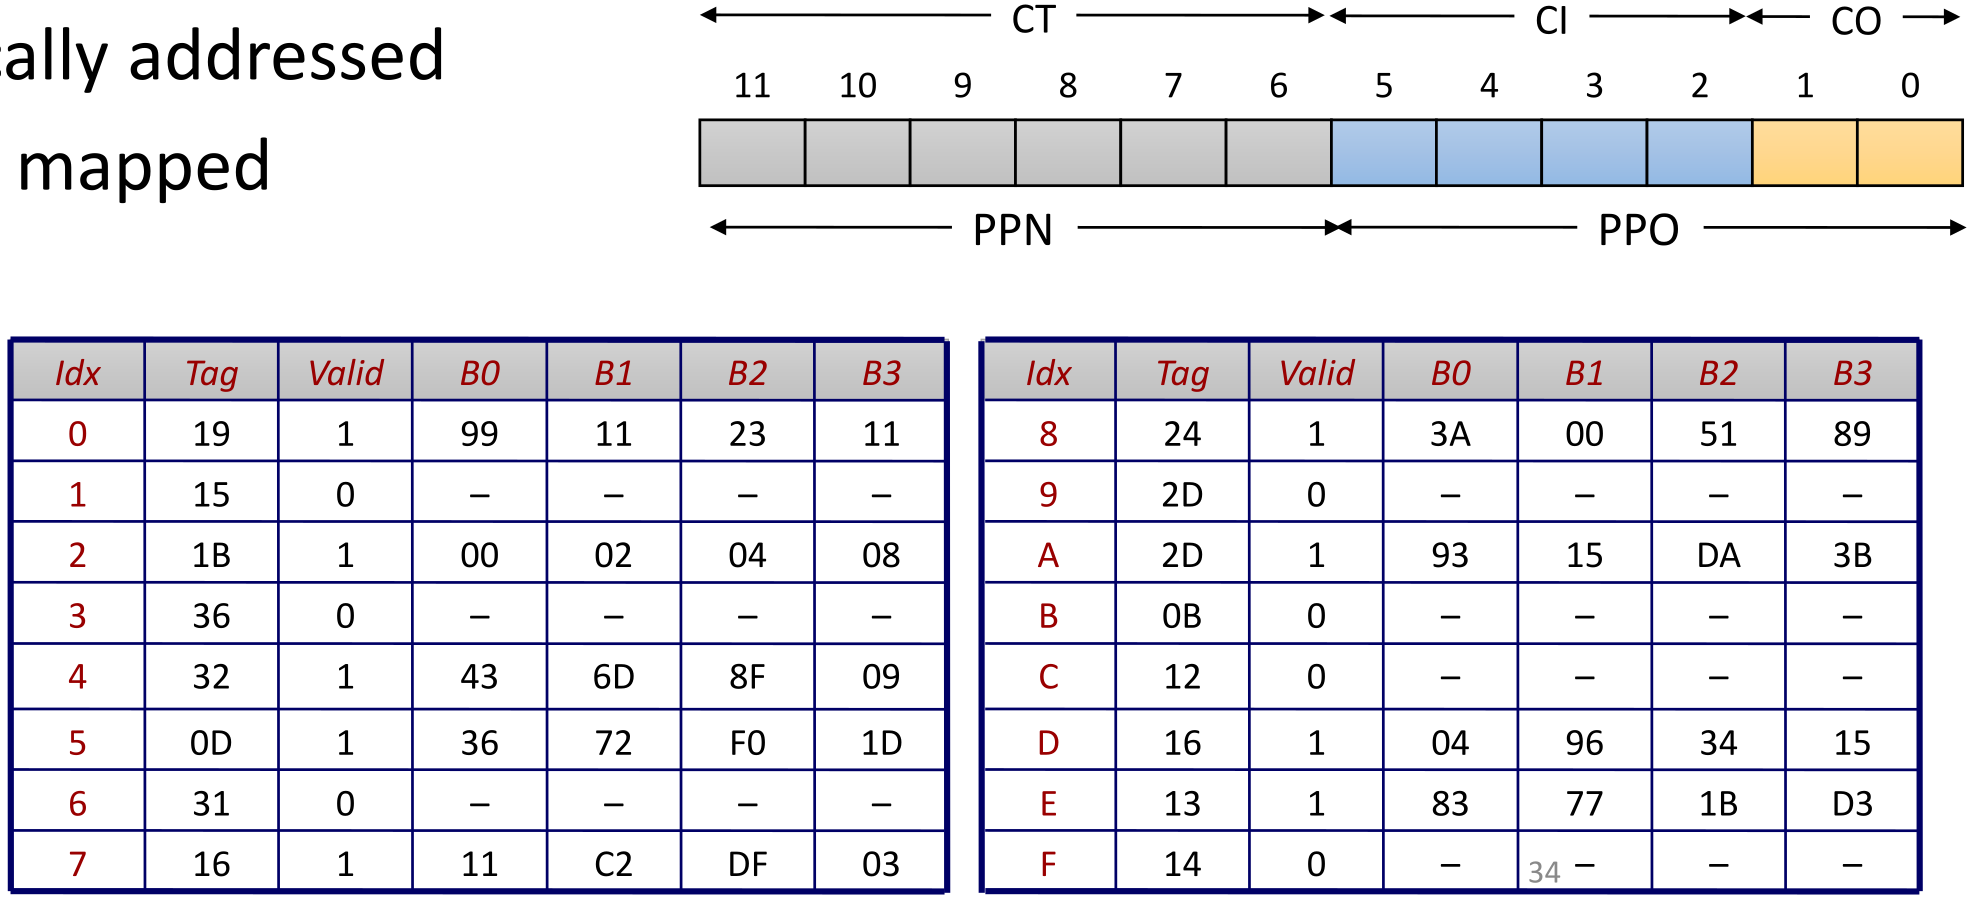
\includegraphics[width=0.8\textwidth]{20_cache.png}

\paragraph{Example 1:}
For the virtual address $0x03D4$ we have:

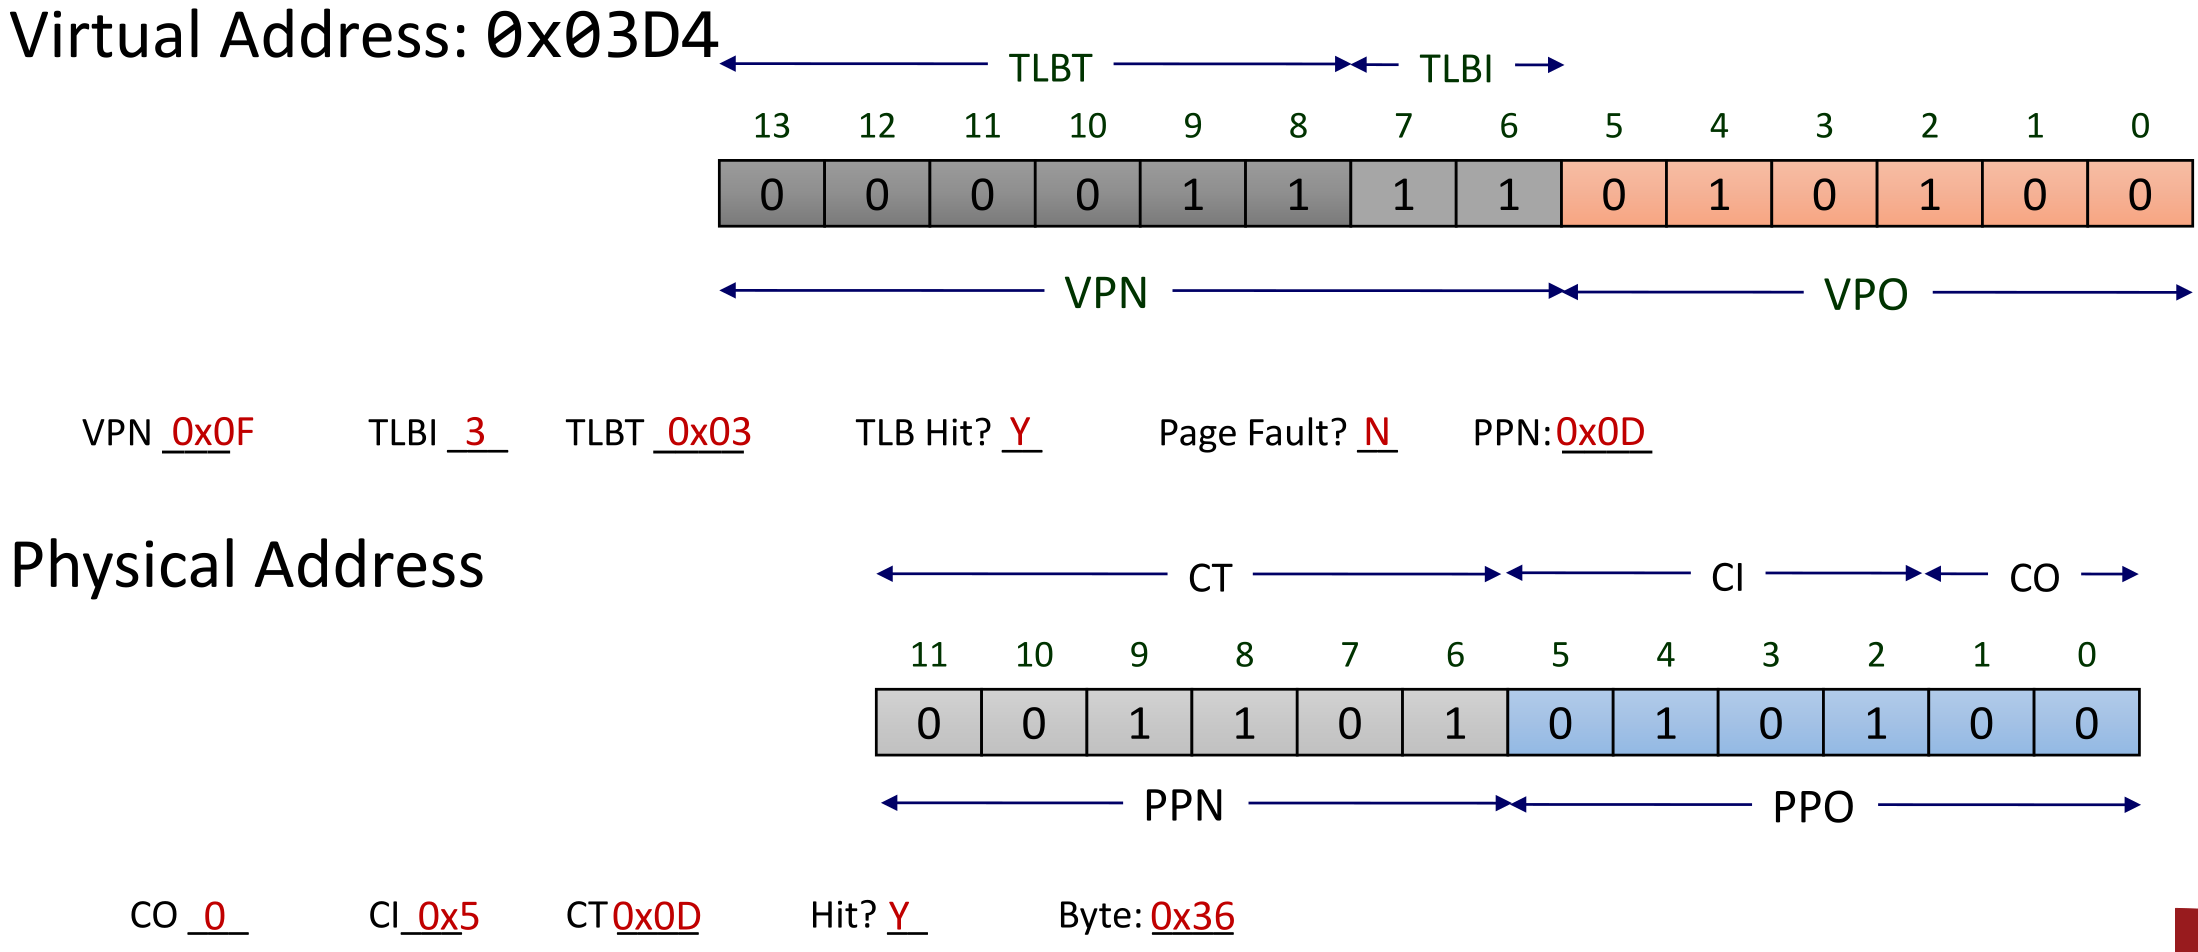
\includegraphics[width=0.8\textwidth]{20_ex1.png}

The PPN is in the TLB and can be retrieved from there. The physical address can be easily constructed and used to access the cache.


\paragraph{Example 2:}
For the virtual address $0x0B8F$ we have:

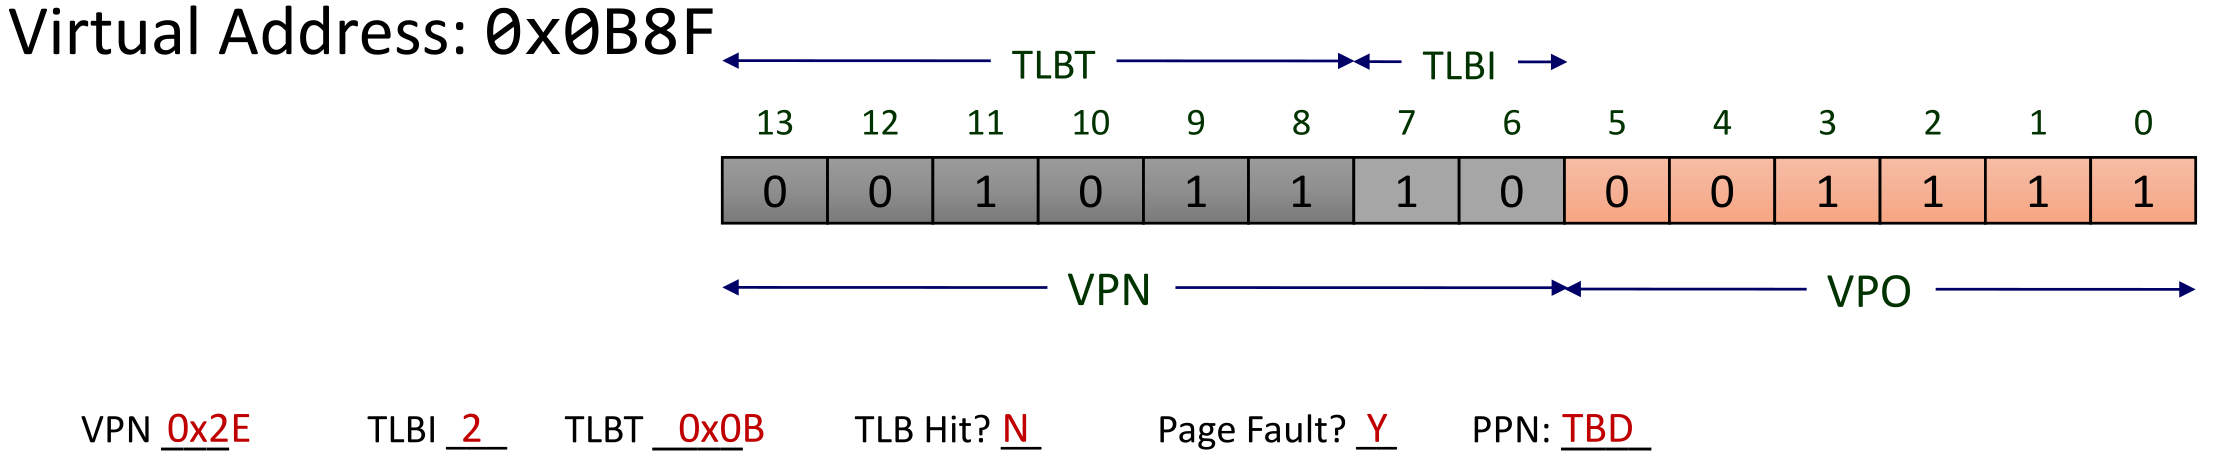
\includegraphics[width=0.8\textwidth]{20_ex2.png}

The PPN is not in the TLB. In this example, the PTE is also not in memory and hence, we get a page fault and is has to be fetched from memory.

\paragraph{Example 3:}
For the virtual address $0x0020$ we have:

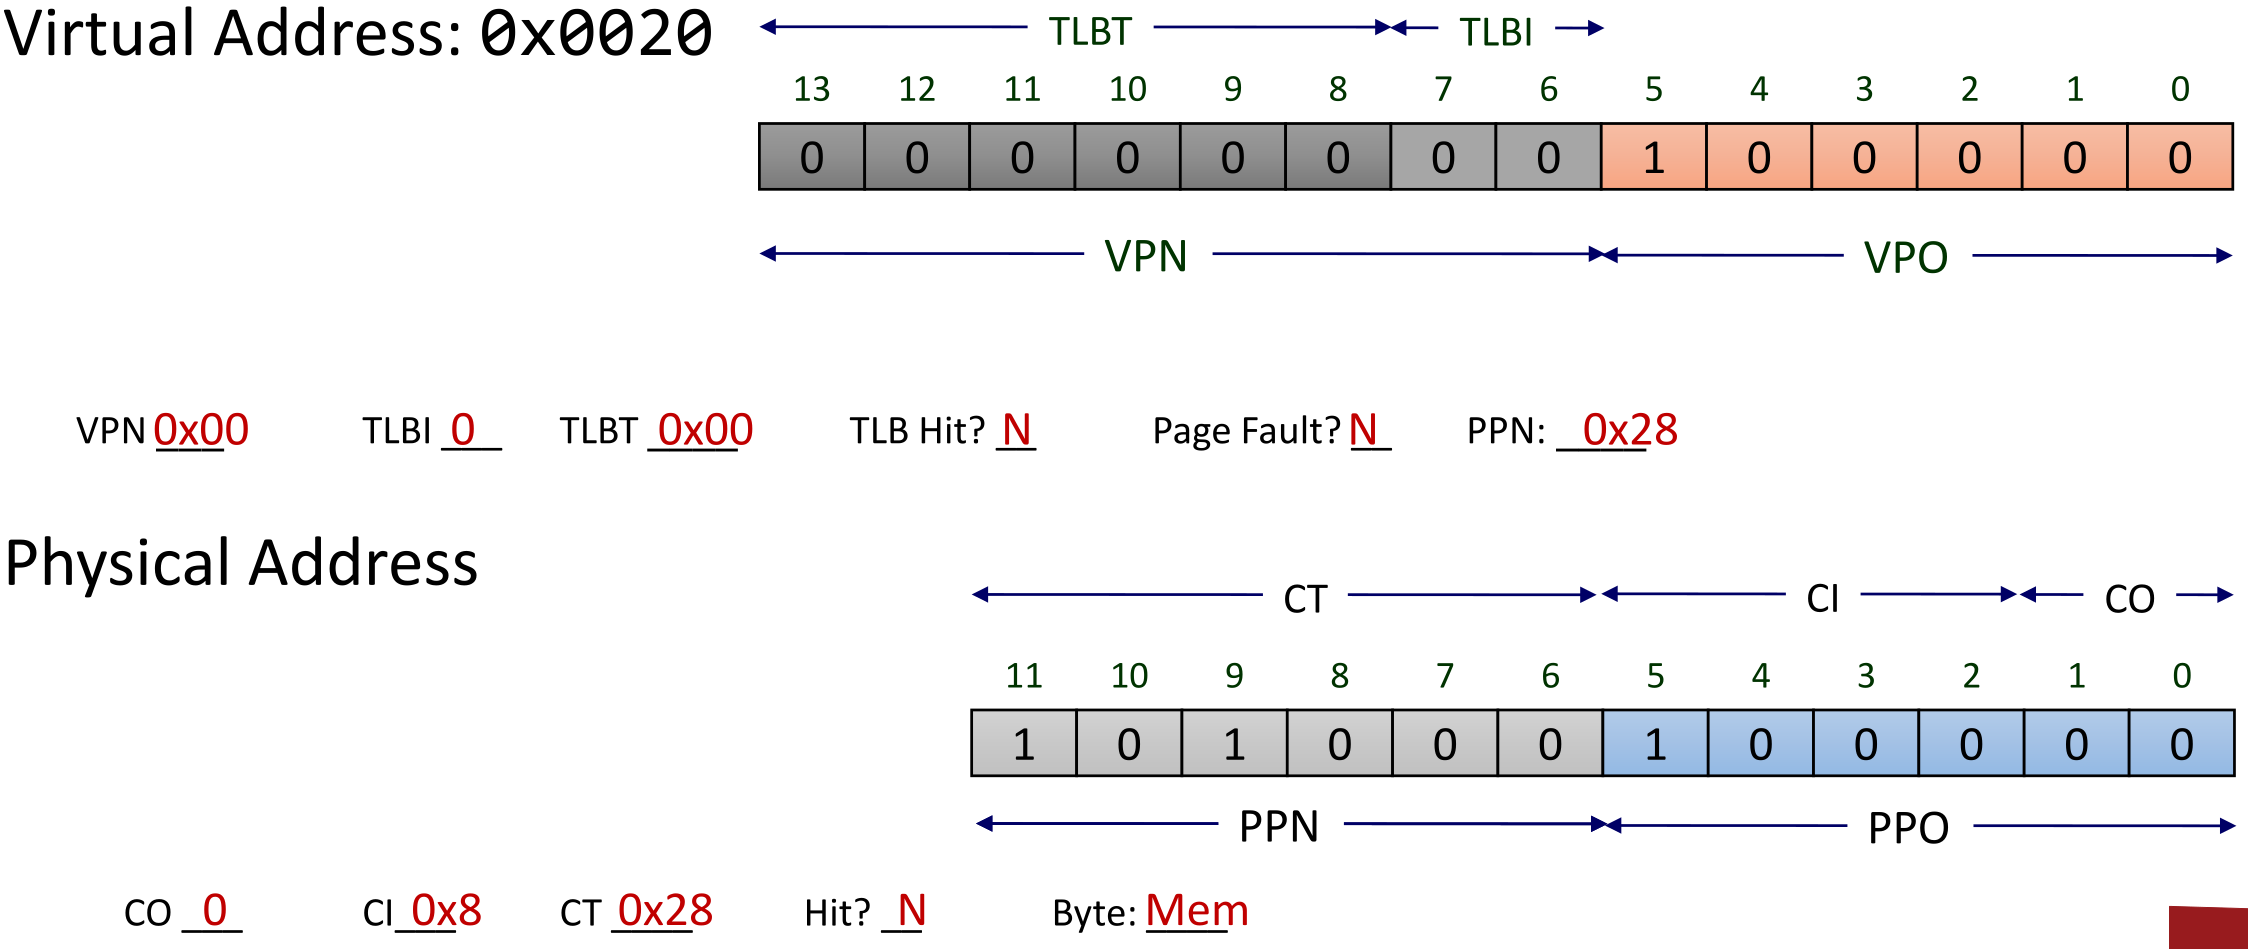
\includegraphics[width=0.8\textwidth]{20_ex3.png}

While the tag is actually in the TLB, it is invalid and hence we do not get a PPN. Therefore, we check in the page table in memory, which is the case for this example.


\textbf{RECHECK: The images of the last two examples are probably wrong}
